\documentclass[11pt]{article}
\usepackage[margin=1in]{geometry}
\usepackage{booktabs}
\usepackage{graphicx}
\usepackage{hyperref}
\usepackage{longtable}
\title{WDS Sentinel: Reliability-Aware Hybrid AI Supervision Under Evidence Degradation}
\author{Naimur Rahman}
\date{September 2026}
\begin{document}
\maketitle

\begin{abstract}
This technical report documents a research prototype that combines a frozen data-driven water-distribution-system (WDS) detector, explicit knowledge-based reasoning, multi-agent orchestration, evidence-quality assessment, selective supervisory control, and grounded explanations. The primary experiment uses public BattLeDIM/L-Town SCADA data and preserves predictive null/weak results rather than hiding them. An independent precipitation stream exercises heterogeneous hazard-context integration, while a final Battle of Water Demand Forecasting (BWDF) extension provides physically co-located real-WDN weather and DMA inflow evidence for observational extreme-rain demand-response validation. Reliability results are reported jointly with autonomous coverage, and no rainfall-to-pipe-failure causal claim is made.
\end{abstract}

\section{System}
The executed WDS chain is: heterogeneous pressure/flow/level evidence $\rightarrow$ frozen predictive score $\rightarrow$ typed evidence state $\rightarrow$ explicit knowledge rules $\rightarrow$ reliability gate $\rightarrow$ supervisory decision and grounded explanation. Evidence, Prediction, Knowledge/Reasoning, Reliability, Hazard and Supervisory agents communicate through typed message contracts. The final WDS action space is \texttt{NO\_ALERT}, \texttt{ALERT}, \texttt{ABSTAIN}, \texttt{ESCALATE}.

\section{Data and protocol}
The main experiment uses 2018 BattLeDIM pressure, flow, level and leakage data at five-minute resolution. January--June is used for training and July--December for validation. The target marks the first hour after a new leak onset. The frozen predictor is a class-balanced logistic regression over causal change features. Four deterministic evidence degradations are added to the clean condition: a fixed missing-sensor subset, additive noise, conflicting flow evidence and stochastic sensor dropout using a fixed seed.

\section{Systems}
System A applies the predictor threshold directly. System B additionally requires independent statistical sensor corroboration. System C applies the same hybrid decision and then invokes a reliability gate based on missingness, cross-modality disagreement and instability. If evidence is unreliable, a base \texttt{ALERT} becomes \texttt{ESCALATE}; a base \texttt{NO\_ALERT} becomes \texttt{ABSTAIN}.

\section{Reliability results}
The 2018 validation set contains 52,980 scored rows and five leak-onset events. System C operates autonomously on approximately 0.83--0.87 of rows in four conditions and on zero rows in the severe fixed missing-sensor condition. Selective unsafe risk is therefore reported only at achieved coverage and is undefined at zero coverage. The results do not support a claim that C has uniformly lower conditional risk when it acts; instead, C makes evidence degradation explicit and can withdraw autonomous decision-making rather than silently continuing.

\begin{figure}[h]
\centering
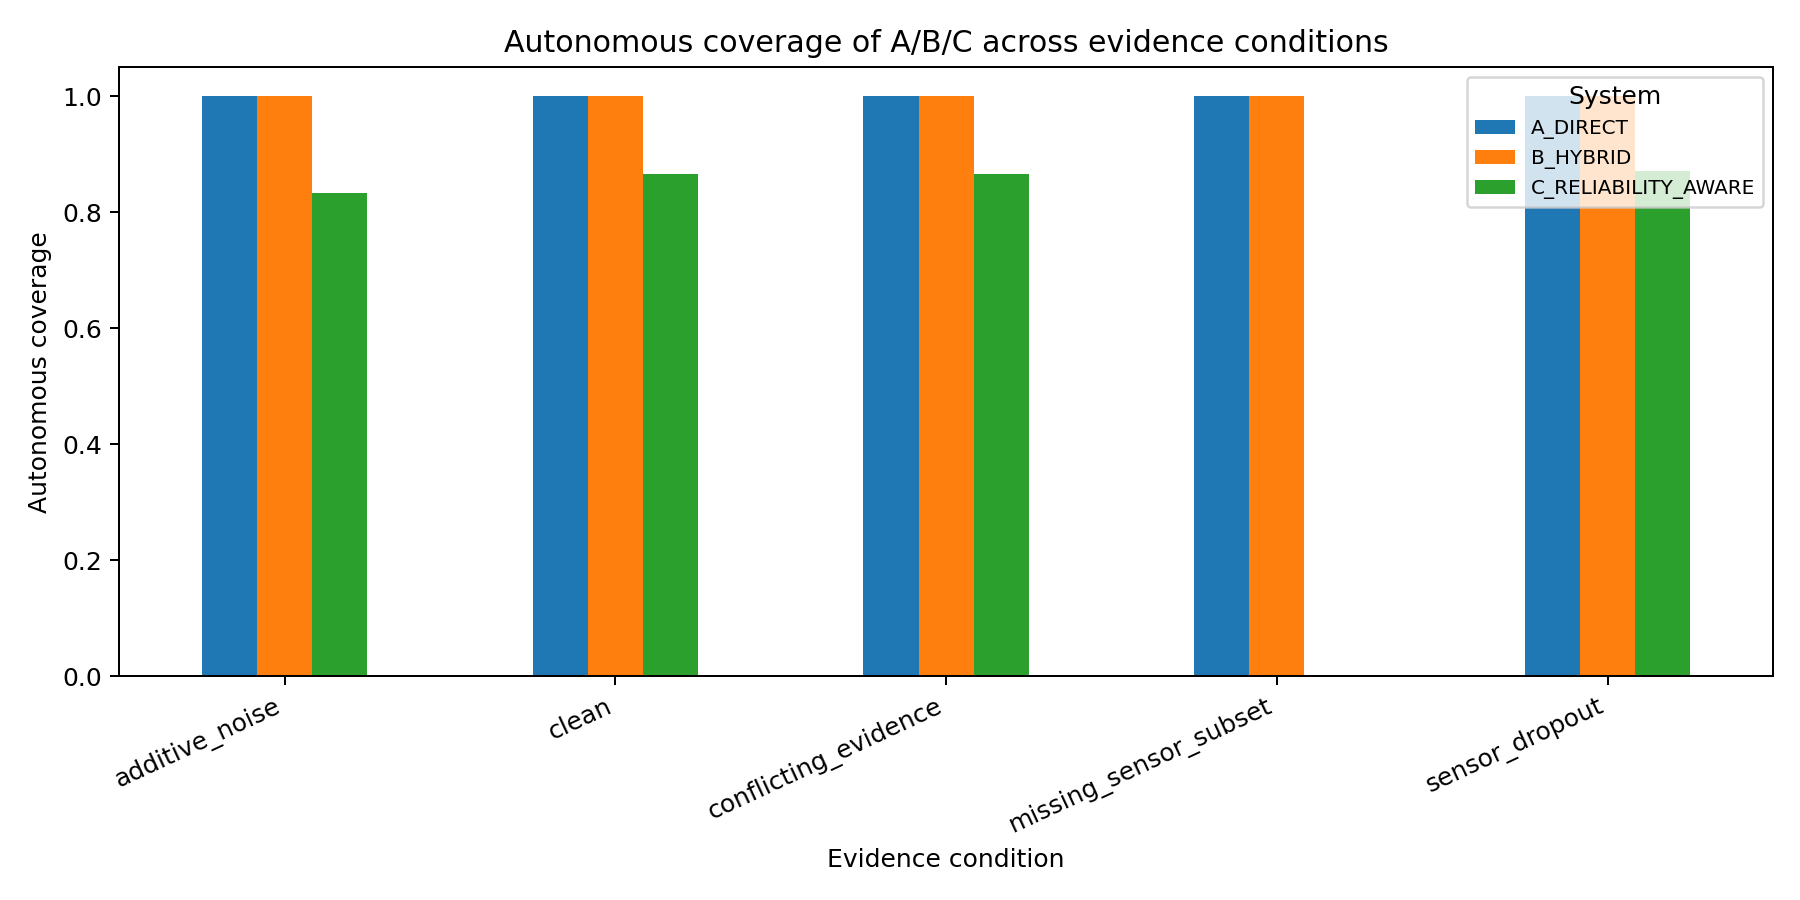
\includegraphics[width=0.92\linewidth]{../results/figures/abc_coverage_by_condition.png}
\caption{Autonomous coverage across evidence conditions.}
\end{figure}

The independent agent implementation reproduces the frozen System-C path exactly on all 52,980 validation rows under each of five evidence conditions: 264,900/264,900 row-level decision matches.


\section{Final temporal evaluation}
After the architecture, predictor, thresholds, degradation definitions and reliability cutoffs were frozen, the complete multimodal system was evaluated on 2019 BattLeDIM pressure, flow and level data. The four 2019 modalities contain 105,120 aligned rows; the frozen detection split applies a one-hour boundary embargo, leaving 105,108 scored rows. Nineteen genuine new onsets are evaluated, while four leaks already active at the first 2019 row are treated as carryovers rather than new events.

The 2019 period is not described as a pristine blind test because pressure/leakage had previously been inspected once by a rejected one-hour-ahead forecasting baseline. No 2019 result was used for subsequent detector, KBS/MAS, or reliability-controller development, and no setting was changed after this final temporal run.

On clean 2019 data the frozen predictor obtains AUPRC 0.004041 and AUROC 0.530564, with precision 0.022161, recall 0.032389 and F1 0.026316 at the frozen threshold 0.99. Systems A, B and C each detect only 1 of 19 new onsets. System C has autonomous coverage 0.8617 and selective unsafe risk 0.002484, compared with 0.002274 for A and 0.002331 for B. Thus the final temporal result does not support strong leak-detection performance or lower conditional risk for C; it supports only the narrower conclusion that the explicit reliability gate continues to expose/withdraw decisions under evidence-quality violations while the predictive substrate remains weak.

\begin{figure}[h]
\centering
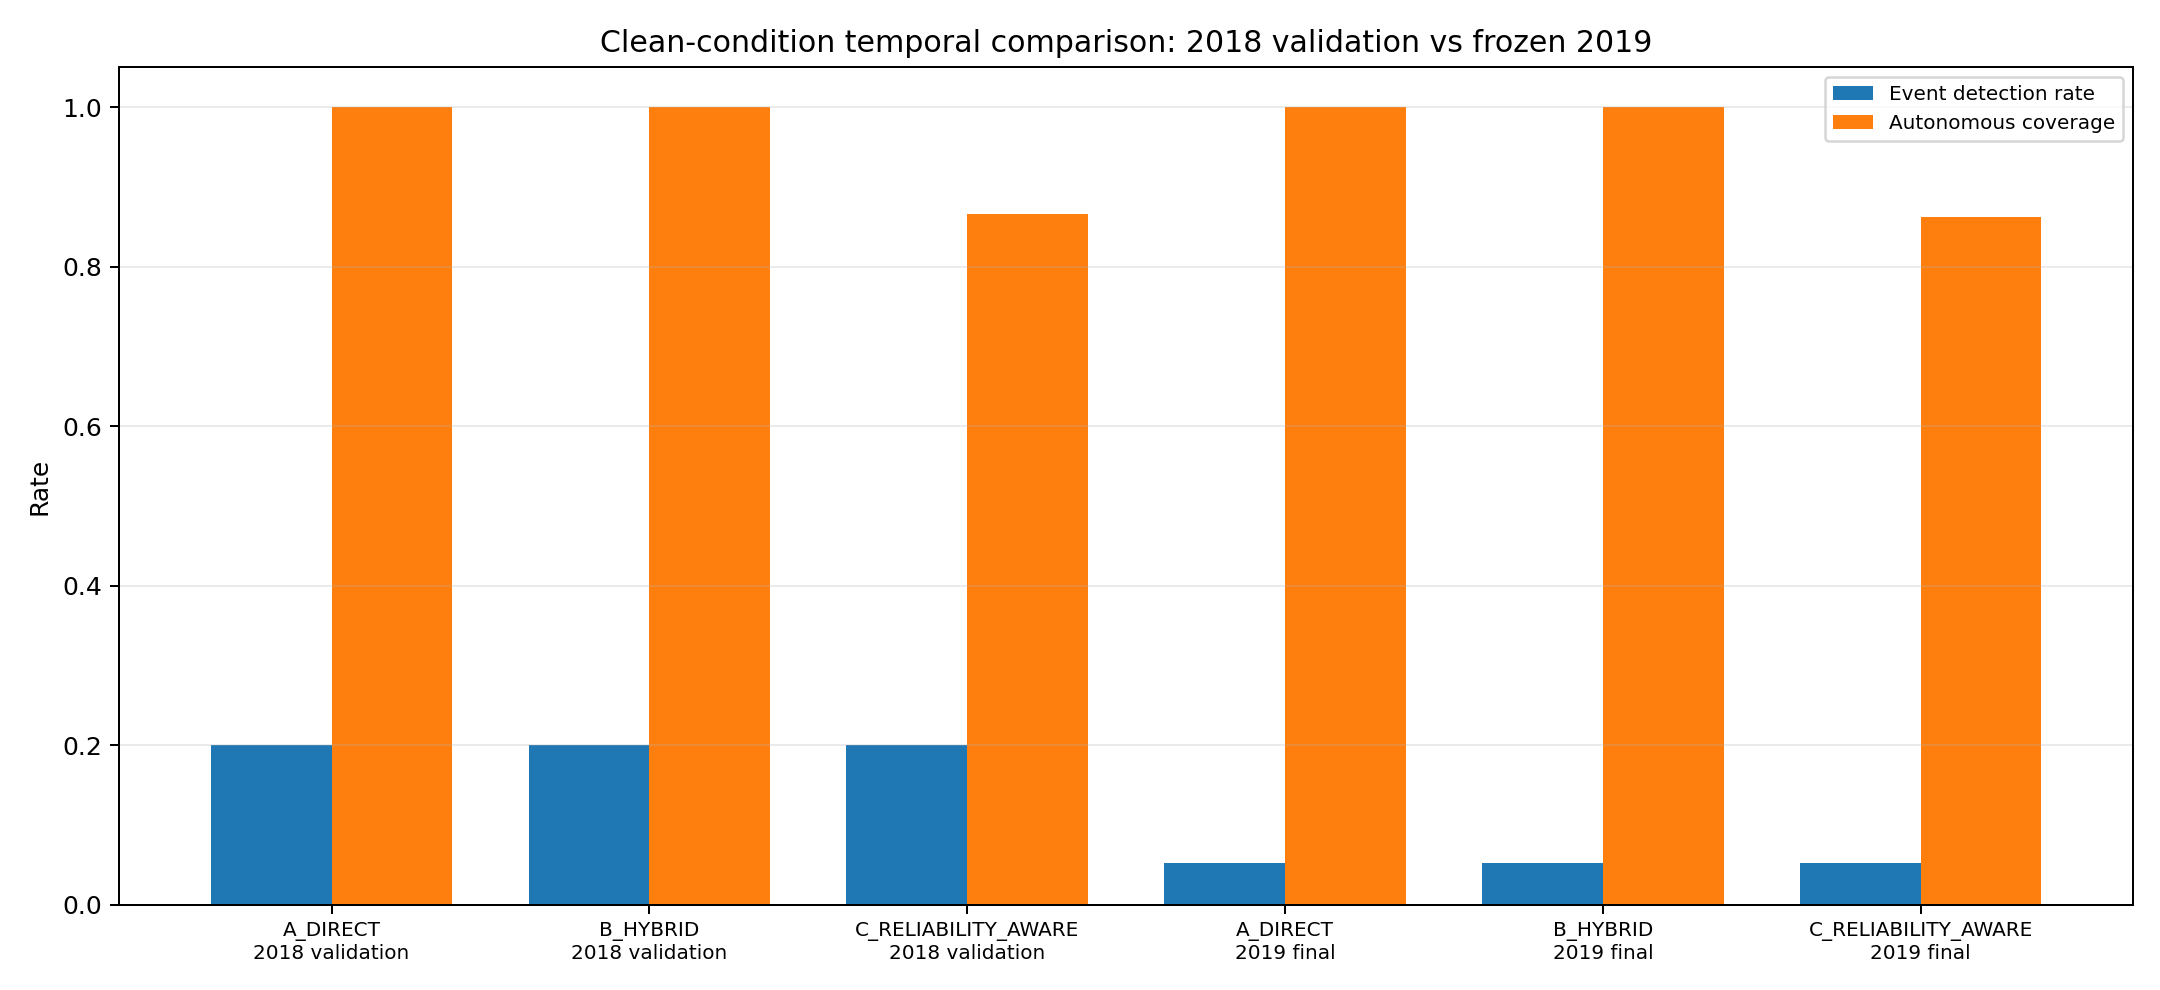
\includegraphics[width=0.92\linewidth]{../results/figures/final_2019_clean_temporal_comparison.png}
\caption{Clean-condition 2018 validation versus final frozen 2019 temporal evaluation.}
\end{figure}

\section{Independent precipitation context}
Daily precipitation observations ultimately originate from Taiwan CWA/CODIS and are used only as an independent evidence stream. A training-calibrated multi-window indicator marks a day elevated when any trailing 1-, 3- or 7-day precipitation sum exceeds its 2013--2017 training 95th-percentile cutoff. Source-documented trace precipitation code $-9.8$ is converted to 0.09 mm. The resulting cutoffs are 34.1 mm, 82.0 mm and 163.575 mm, respectively; 21 of 365 days in 2018 are flagged elevated. This is not a flood/damage classifier.

\section{Integrated real-evidence scenarios}
The integrated scenario exporter selects actual BattLeDIM validation rows rather than authoring WDS values by hand. It uses a genuine normal/no-onset row, a genuine onset-window row actually detected by the frozen system, and a genuine degraded onset-window row that invokes the reliability gate. These are paired, as independent contexts, with actual normal/elevated precipitation observations. The integrated agent supports separate WDS and hazard timestamps so the unrelated datasets are never presented as temporally aligned.

\begin{figure}[h]
\centering
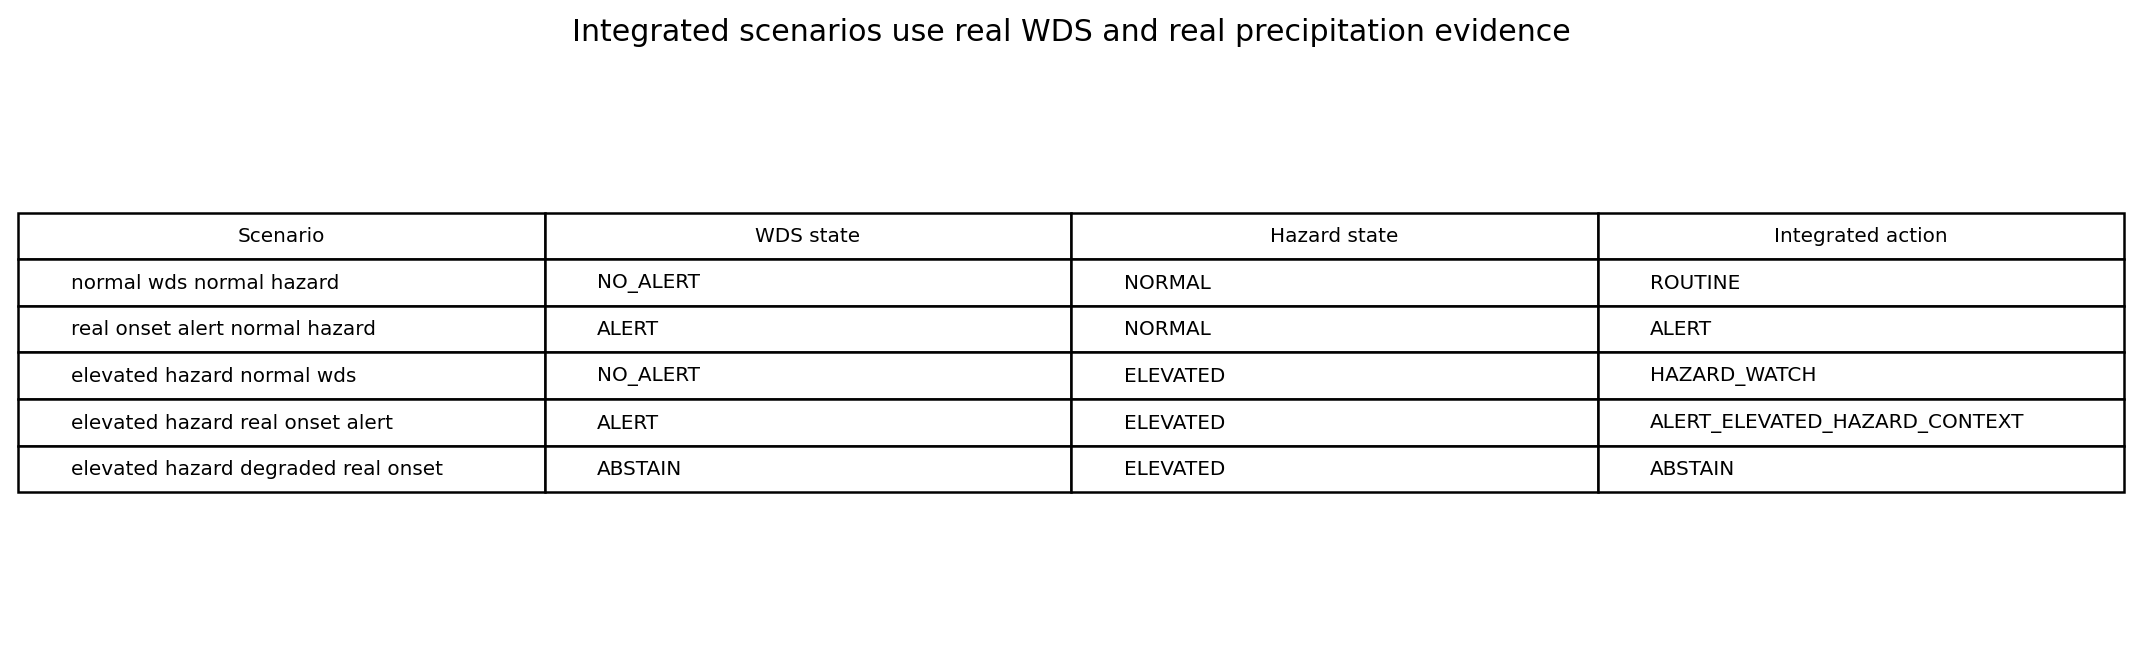
\includegraphics[width=0.98\linewidth]{../results/figures/integrated_real_evidence_scenarios.png}
\caption{Integrated actions from real evidence on both input streams.}
\end{figure}

\section{Physically linked extreme-weather / WDN validation}
The final extension uses the Battle of Water Demand Forecasting (BWDF) supplementary data from a real WDN in northeast Italy. The bundled workbooks contain 19,679 aligned hourly observations from January 2021 through March 2023: net inflow for ten DMAs and rainfall, temperature, humidity and wind from a weather station located within the same case-study WDN. The files are distributed under CC BY 4.0 and were verified byte-for-byte against the public \texttt{WaterFutures/wf4bwdf} repository.

The frozen linked-weather protocol trains through 2022-07-24 23:00 Europe/Rome and evaluates BWDF week W1 (2022-07-25--31). The original BWDF protocol supplied weather observations for each evaluation week as a perfect weather forecast, so W1 weather is a legitimate exogenous input rather than future leakage under that benchmark. A simple Ridge model with 168-hour and 336-hour demand lags, calendar cycles, and current W1 weather is compared against a same-hour previous-week baseline. A training-only 95th percentile of positive daily rainfall totals defines extreme rain; the resulting threshold is 18.775 mm/day.

The weather-aware model has lower W1 MAE than the previous-week baseline in 9 of 10 DMAs. For the two pre-specified summer-rain-sensitive residential DMAs identified by the BWDF publication, DMA 2 improves from 1.8261 to 1.4723 L/s MAE (19.4\%) and DMA 3 improves from 1.5626 to 1.3333 L/s (14.7\%). Across the post-training period, 11 extreme-rain days and 148 dry days are available. The mean same-hour previous-week demand residual on extreme-rain days is lower than on dry days by 0.432 L/s in DMA 2 (descriptive bootstrap 95\% interval [-0.778, -0.141]) and 0.530 L/s in DMA 3 ([-0.966, -0.188]).

Actual co-located weather and demand evidence are exported as typed evidence objects and evaluated by explicit rules. On the first post-training extreme-rain day, both pre-specified DMAs fire \texttt{R8\_EXTREME\_RAIN}, \texttt{R9\_DEMAND\_SUPPRESSION}, and \texttt{R10\_LINKED\_WEATHER\_RESPONSE}, producing \texttt{WEATHER\_LINKED\_DEMAND\_RESPONSE}. This establishes a physically linked observational weather--WDN operational response; it does not establish rainfall-caused hydraulic failure.

\begin{figure}[h]
\centering
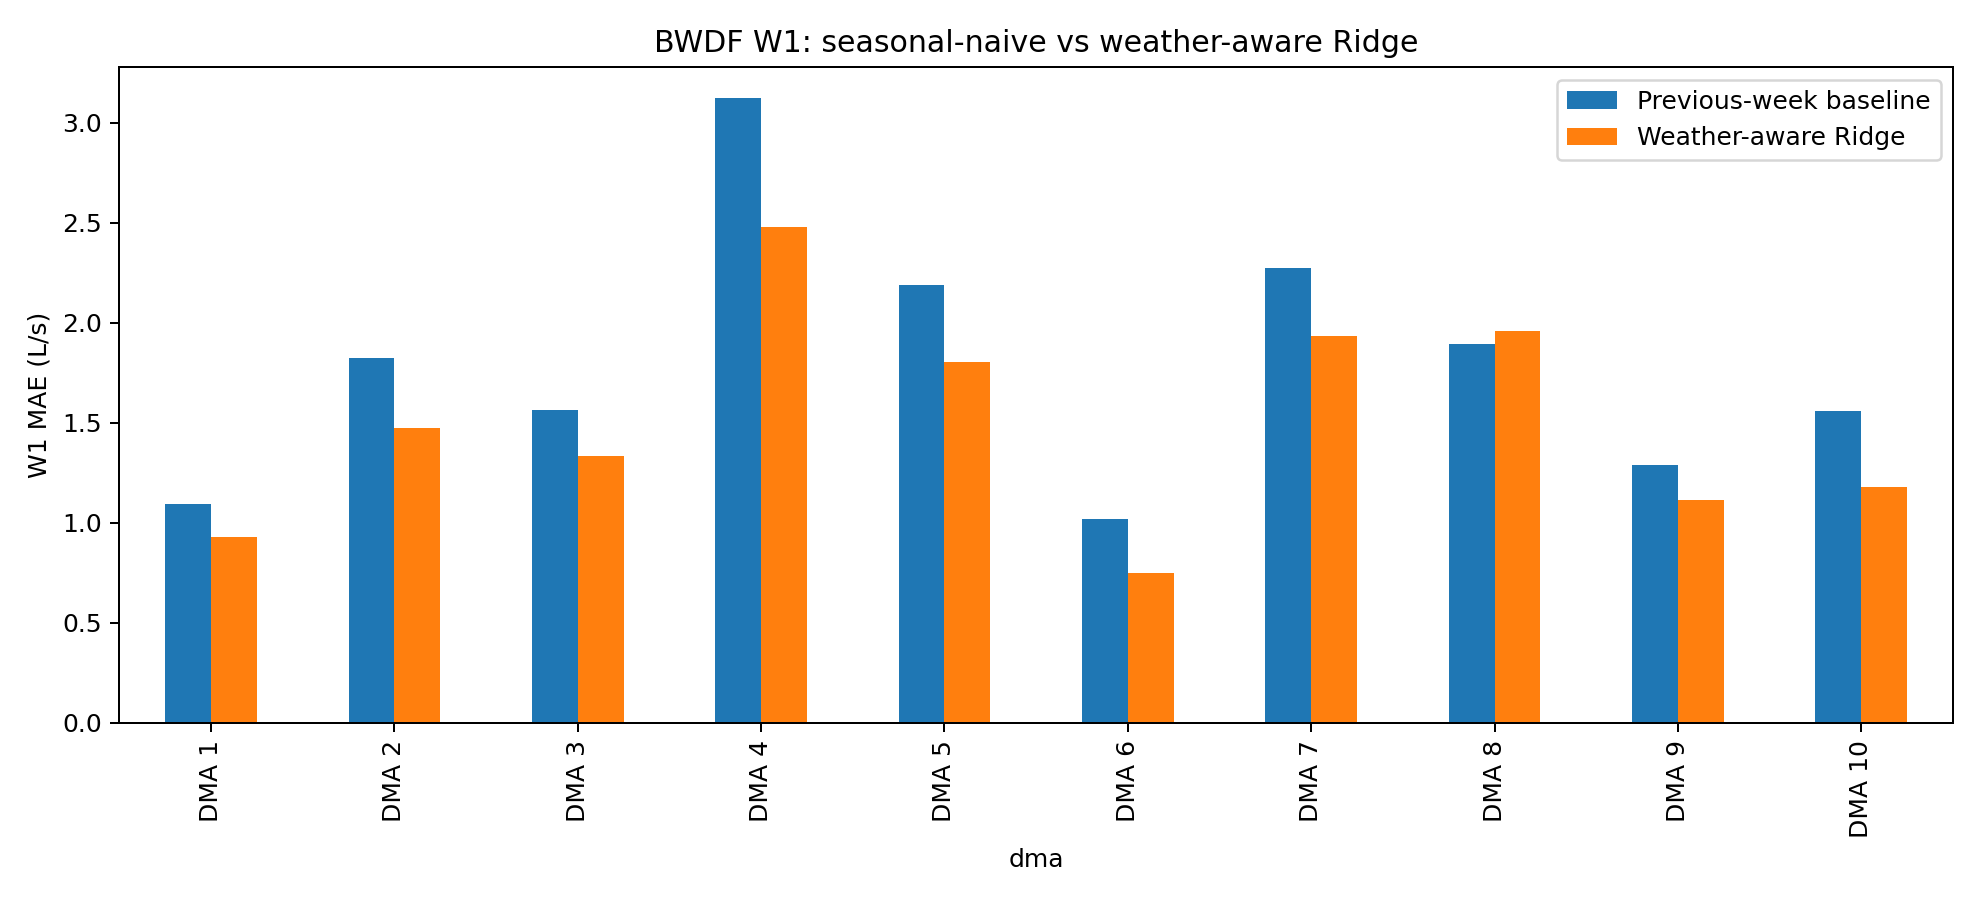
\includegraphics[width=0.92\linewidth]{../results/figures/linked_bwdf_w1_forecast_comparison.png}
\caption{BWDF W1 comparison of previous-week and weather-aware demand forecasts.}
\end{figure}

\begin{figure}[h]
\centering
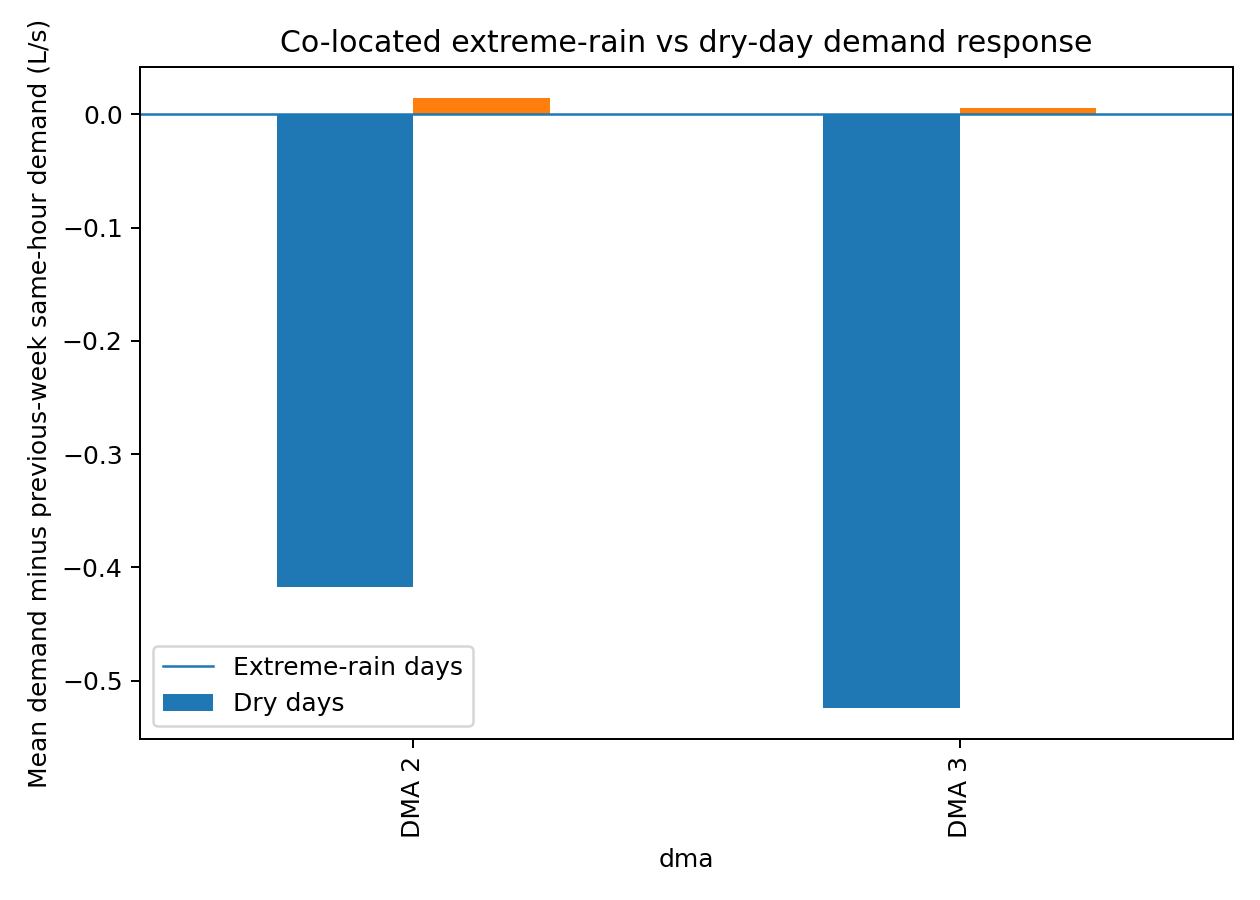
\includegraphics[width=0.78\linewidth]{../results/figures/linked_bwdf_extreme_rain_response.png}
\caption{Co-located extreme-rain versus dry-day weekly demand residuals for the pre-specified weather-sensitive DMAs.}
\end{figure}

\section{Limitations}
The predictor is weak and is not operationally validated. Only five validation onsets occur in the selected 2018 split, and the final clean 2019 run detects only 1 of 19 new onsets. The CWA/CODIS hazard-context stream is independent of L-Town and does not establish hydraulic consequences. The separate BWDF extension establishes a real co-located weather--demand response, but it remains observational and does not establish rainfall-caused hydraulic failure. Four leaks carry over into 2019 and are excluded from the new-onset target; therefore alert burden outside new-onset windows is not necessarily operationally equivalent to a false leak indication. Dataset ownership remains with the original publishers; rights/provenance notes are separated from the MIT-licensed project code.

\section{Reproducibility}
The repository includes source code, tests, data provenance, bundled experiment data, derived outputs and raw run logs. The final audited automated suite contains 135 passing tests. Reproduction entry points and direct dependency snapshots are documented in the repository README.

\end{document}
